\documentclass[12pt,spanish]{article}
\usepackage[utf8]{inputenc}
\usepackage[spanish]{babel} 
\usepackage[utf8]{inputenc}	
\spanishdecimal{.}
\usepackage{amsmath,amsthm,amsfonts,amssymb,amscd}
\usepackage{multirow,booktabs}
\usepackage[table]{xcolor}
\usepackage{fullpage}
\usepackage{lastpage}
\usepackage{enumitem}
\usepackage{fancyhdr}
\usepackage{mathrsfs}
\usepackage{wrapfig}
\usepackage{setspace}
\usepackage{graphicx}
\usepackage[retainorgcmds]{IEEEtrantools}
\usepackage[margin=3cm]{geometry}
\newlength{\tabcont}
\usepackage{algorithm}
\usepackage{algorithmic}
\setlength{\parindent}{0.0in}
\setlength{\parskip}{0.05in}



\title{Taller No. 1 Complejidad}

\newcommand\course{Análisis De Algoritmos}	
\newcommand\semester{2016}  
\newcommand\asgnname{2}        
\newcommand\yourname{David Calle, Carlos Silva, David Suárez}
\newcommand{\vect}[1]{\overline{#1}}
\newcommand{\norm}[1]{\left\lVert#1\right\rVert}
\theoremstyle{definition}
\newtheorem{defn}{Definición}
\newtheorem{reg}{Regla}
\newtheorem{ejer}{EJERCICIO}
\pagestyle{fancyplain}
\headheight 32pt
\lhead{\yourname\ \vspace{0.1cm} \\ \course}
\chead{\textbf{\Large Complejidad}}
\rhead{2016/10/02}
\cfoot{P\'agina \thepage \hspace{1pt} de \pageref{LastPage} \vspace{3mm} \\ \footnotesize \textcolor{gray}{Análisis De Algoritmos, Leonardo Flórez}}
\textheight 580pt
\headsep 10pt
\footskip 40pt
\topmargin = 7pt



\begin{document}

%----------------------------------------------------------
% --------------- Insertion Sort -------------------------
%----------------------------------------------------------

\section{Insertion Sort}{}

% ----------------- Definición Formal ---------------------
\subsection{Formalmente:}{}
Entradas: Una secuencia $S$ con $N$ números:
\begin{equation}
    S =  \left.\langle a_{1}, a_{2}, a_{3}, \cdots, a_{N} \rangle\right.;
    N > 0
\end{equation}

Salidas: Una secuencia $S$ con $N$ números tal que:
\begin{equation}
     S =  \left.\langle  a_{1} \le a_{2} \le, \cdots, \le a_{N} \rangle\right.;
\end{equation}

% ----------------- Pseudocódigo --------------------------
\subsection{Pseudocódigo:}{}
\begin{algorithm}
\begin{algorithmic}[1]
\STATE \textbf{function} InsertionSort( $S$ ) 
\FOR {$i \leftarrow 2$ \textbf{to} $|S|$}
    \STATE $k \leftarrow S[j]$
    \STATE $i \leftarrow j - 1$
    \WHILE{ $ i > 0 \wedge	 S[i] > k$ }
        \STATE $ S[i+1] \leftarrow S[i]$
        \STATE $ i \leftarrow i-1$
    \ENDWHILE
    \STATE $ S[i+1] \leftarrow k$
\ENDFOR
\RETURN $S$
\STATE \textbf{end function}
\caption{Insertion Sort.}
\end{algorithmic}
\end{algorithm}

% ----------------- Invariantes --------------------------
\subsection{Invariantes:}{}
Se puede encontrar una invariante en este algoritmo.
\subsubsection{En cada iteración \textbf{for} la secuencia entre $1$ y $j-1$ siempre está ordenada:}{}

\begin{enumerate}
\item Formalmente: $S \left.\langle a_{1}, a_{2}, a_{3}, \cdots, a_{N-1} \rangle\right. \equiv S' \left.\langle a_{1}, a_{2}, a_{3}, \cdots, a_{N-1} \rangle\right. $
Donde $S' | a_{1} \le a_{2} \le, \cdots, \le a_{N} $

\item Prueba por inducción:
    \begin{enumerate}
    \item Inicialización ( $i \leftarrow 1 $ ):\\
        En la primera iteración del ciclo se cumple que: $ S \equiv S' $ ya que es un único elemento y un elemento por definición siempre está ordenado. 
    \item Mantenimiento/Iteración/Actualización/Procesamiento  ($ 2  \le i  \le N $):\\
        Debido a la condición del ciclo \textbf{while} se controla que los números mayores a $k = S[j]$ queden en las posiciones $ j, j + 1, j+2, \cdots, N $ y los menores o iguales a $k$ en las posiciones $j-1, j-2, \cdots, 1$.
    \item Terminación ($ i \leftarrow N $): \\
        Al terminar el algoritmo $S$ está ordenado.
    \end{enumerate}
\end{enumerate}

% ----------------- Análisis de Complejidad Temporal --------------
\subsection{ Análisis de Complejidad Temporal:}
\subsubsection{Peor caso:}{}
Para el algoritmo Insertion Sort el peor de los casos es que tenga que organizar cada uno de los elementos que están en el vector repitiéndose $n$ veces en el ciclo \textbf{for} y $n$ veces en el  ciclo \textbf{while}. Hay que tener en cuenta que entre la secuencia este más ordenada cuando llega el algoritmo a de ser más demorado por consiguiente la complejidad queda:

$T(n)= \left\{ \begin{array}{lcc}
              c \hspace{0.5cm}  n \leq 0 \\
              \\ nT(1) +cn \hspace{0.5cm} n \geq 1 \\
              \end{array}
    \right.$ \\ \\
$T(n) = O(n^{2})$

\subsubsection{Mejor caso:}{}
Para el algoritmo Insertion Sort el mejor de los casos es que no entre al ciclo \textbf{while}, es decir, que llegue la secuencia ya ordenada por lo cual solo haría $n$ veces el recorrido en la secuencia organizándola. La complejidad quedaría:

$T(n)= \left\{ \begin{array}{lcc}
              c \hspace{0.5cm}  n \leq 0 \\
              \\cn \hspace{0.5cm} n \geq 1 \\
              \end{array}
    \right.$ \\ \\
$T(n) = \Omega (n)$

% ----------------- Análisis de Complejidad Espacial --------------
\subsection{ Análisis de Complejidad Espacial:}
Para todos los casos, Insertion Sort tiene una coplejidad espacial $O(1)$, ya que al no hacer ningún cambio, no debe crear espacio en memoria. Asumiendo que se le reserva memoria una sola vez a $k$.

% ----------------- Análisis de Complejidad --------------
\subsection{ Análisis Práctico:}
Para analizar la teoría anteriormente establecida en casos prácticos se tomaron arreglos de tamaño 1 hasta 1000. Y se puso a prueba el algoritmo Insertion Sort para ordenar estos arreglos en tres escenarios distintos: Cuando todos los arreglos estaban ya ordenados ascendentemente (ordenado), ordenados descendentemente (desordenado) y mezclados, es decir, números aleatorios (aleatorio). Posteriormente se graficó, tamaño (n) vs tiempo (seg), el comportamiento de este algoritmo en los tres escenarios obteniendo la siguiente gráfica:

\begin{figure}[htb]
\centering
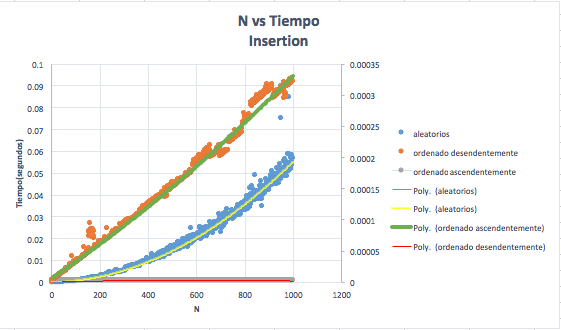
\includegraphics[scale=0.6]{I}
\caption{Comportamiento algoritmo Insertion Sort.}
\end{figure}

Insertion Sort es un algoritmo que depende de los datos que vengan en el vector que se va a organizar. Es decir si el vector que recibo ya esta todo organizado este será mucho mas eficiente como se puede ver en la línea gris de la grafica de Insertion donde el tiempo es constante a diferencia si el vector que se recibe tiene parcialmente números ordenados se puede notar que el algoritmo demorara más tiempo como se observa en el conjunto de datos color azul de la misma grafica. Finalmente si los datos están totalmente desordenados este algoritmo demorara muchos mas tiempo que los dos casos anteriores como se ve en la grafica naranja. 
%----------------------------------------------------------
% --------------- Merge Sort -------------------------
%----------------------------------------------------------

\section{Merge Sort}{}

% ----------------- Definición Formal ---------------------
\subsection{Formalmente:}{}
Entradas: Una secuencia $S$ con $N$ números:
\begin{equation}
    S =  \left.\langle a_{1}, a_{2}, a_{3}, \cdots, a_{N} \rangle\right.;
    N > 0
\end{equation}

Salidas: Una secuencia $S$ con $N$ números tal que:
\begin{equation}
     S =  \left.\langle  a_{1} \le a_{2} \le, \cdots, \le a_{N} \rangle\right.;
\end{equation}

% ----------------- Pseudocódigo --------------------------
\subsection{Pseudocódigo:}{}

\begin{algorithm}
\begin{algorithmic}[1]
\STATE \textbf{procedure} MergeSort( $S, f, l$ ) 
\IF {$f < l$ }
    \STATE $h \leftarrow \lfloor (f+l)/2 \rfloor$
    \STATE MergeSort( $S, f, h$ ) 
    \STATE MergeSort( $S, h+1, l$ ) 
    \STATE Merge( $S, f, h,l$ ) 
\ENDIF
\STATE \textbf{end procedure}
\caption{Merge Sort.}
\end{algorithmic}
\end{algorithm}

\begin{algorithm}
\begin{algorithmic}[1]
\STATE \textbf{procedure} Merge( $S, p, q, r$ ) 
\STATE $n_{1} \leftarrow q-p+1$
\STATE $n_{2} \leftarrow r-q$
\STATE \textbf{Let} $L[1,n_{1}+1]$ \textbf{and} $R[1,n_{2}+1]$
\FOR{$i \leftarrow 0 \hspace{0.2cm} \textbf{to} \hspace{0.2cm} n_{1}$ }
    \STATE $L[i] \leftarrow S[p+i-1]$
\ENDFOR

\FOR{$i \leftarrow 0 \hspace{0.2cm} \textbf{to} \hspace{0.2cm} n_{2}$ }
    \STATE $R[i] \leftarrow S[q+j]$
\ENDFOR

\STATE $L[n_{1}+1] \leftarrow \infty \wedge R[n_{2}+1] \leftarrow \infty$
\STATE $i\leftarrow 1 \wedge j \leftarrow 1 $
\FOR{$k \leftarrow p \hspace{0.2cm} \textbf{to} \hspace{0.2cm}r$ }
    \IF{$L[i] \le R[j]$}
        \STATE $S[k] \leftarrow L[i]$
        \STATE $i \leftarrow i+1$
    \ELSE
        \STATE $S[k] \leftarrow R[j]$
        \STATE $j \leftarrow j+1$
    \ENDIF
\ENDFOR
\STATE \textbf{end procedure}
\caption{Merge.}
\end{algorithmic}
\end{algorithm}

\clearpage
% ----------------- Invariantes --------------------------
\subsection{Invariantes:}{}
Se puede encontrar una invariante en este algoritmo.
\subsubsection{En cada iteración \textbf{for}, la secuencia $S[p, k–1]$ contiene los $k–$elementos más pequeños entre $L$ y $R$, ordenados. Además, $L[i]$ y $R [j]$ son los valores más pequeños de cada secuencia que no han sido copiados en $S$:}{}

\begin{enumerate}

\item Prueba por inducción:
    \begin{enumerate}
    \item Inicialización:\\
        En la primera iteración del ciclo la secuencia $S[p,k-1]$ con tiene un único elemento que corresponde al más pequeño debido a la condición de la sentencia \textbf{if} que solo deja agegar a esta sentencia el elemneto más pequeño de $L$ o de $R$.
    \item Mantenimiento/Iteración/Actualización/Procesamiento:\\
        A medida que se va ordenando cada mitad recursiva de la secuencia por separado, se tienen las subsecuencias $L$ y $R$ que representan las dos mitades de la secuencia $S$ ordenada por ende el elemento que se copie a $S$ desde $L$ o $R$ se asegura, debido la condición \textbf{if}, que es  el menor entre estas dos subsecuencias.
    \item Terminación ($ i \leftarrow N $): \\
        Al terminar el algoritmo la secuencia $S[p,k-q] \equiv S[N]$  contiene todos los elementos ordenados y las subsecuencias $L$ y $R$ ya no contienen elementos esto aseguro que para llegar a la secuencia $S$ totalmente ordenada se debieron copiar de manera ascendente (primero los más pequeños) los elementos de cada subsecuencia $L$ y $R$.
    \end{enumerate}
 \end{enumerate}

% ----------------- Análisis de Complejidad ------------------------
\subsection{ Análisis de Complejidad Temporal:}
Para este algoritmo de ordenamiento todos los casos (promedio, peor y mejor) son el mismo ya que no existen validaciones de orden para dividir la secuencia y unirla, es decir, así la secuencia esté ordenada Merge Sort la divide y une.
Por lo tanto la complejidad de este algoritmo se define como:

$2T(\frac{n}{2})$ ya que la secuencia se divide en dos y el algoritmo se aplica a cada mitad.

$cn$ es la complejidad ($O(n)$ peor de los casos) para la unión de las dos sub-secuencias. 

$T(n)= \left\{ \begin{array}{lcc}
              c \hspace{0.5cm}  n \leq 0 \\
              \\ 2T(\frac{n}{2}) +cn \hspace{0.5cm} n \geq 1 \\
              \end{array}
    \right.$ \\ \\
$T(n) = \theta \equiv O \equiv \Omega(nlog_{2}(n))$
% ----------------- Análisis de Complejidad Espacial ----------------
\subsection{ Análisis de Complejidad Espacial:}
En cada una de las iteraciones de merge sort para dividir la secuencia $S$ se crea una nueva secuencia  de tamaño $n$. Y teniendo en cuenta lo encotrado en el inciso anterior la cantidad de veces que se repite, en el peor de los casos, es $log_{2}(n)$ (altura del árbol), por lo que el total de tamaño extra tomado es, para las tres complejidades, de $O(nlog_{2}(n))$.
% ----------------- Análisis de Practico --------------
\subsection{ Análisis Práctico:}
Para analizar la teoría anteriormente establecida en casos prácticos se tomaron arreglos de tamaño 1 hasta 1000. Y se puso a prueba el algoritmo Merge Sort para ordenar estos arreglos en tres escenarios distintos: Cuando todos los arreglos estaban ya ordenados ascendentemente (ordenado), ordenados descendentemente (desordenado) y mezclados, es decir, números aleatorios (aleatorio). Posteriormente se graficó, tamaño (n) vs tiempo (seg), el comportamiento de este algoritmo en los tres escenarios obteniendo la siguiente gráfica:

\begin{figure}[htb]
\centering
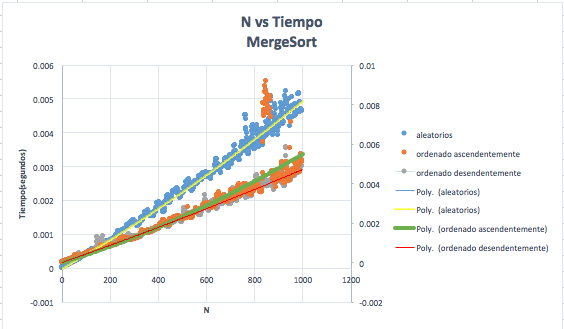
\includegraphics[scale=0.6]{M}
\caption{Comportamiento algoritmo Merge Sort.}
\end{figure}

En el caso de Merge Sort todos lo casos tienen la misma complejidad, esto se puede ver reflejado en la gráfica ya que estás coinciden con la forma de la función $nlogn$. Sin embargo,  es un poco extraño que el aleatorio haya tomado un poco más de tiempo. Esto pudo haber sido causado por cambios en el uso del computador el algoritmo hace exactamente las mismas operaciones para todos los casos.
%----------------------------------------------------------
% --------------- Quick Sort -------------------------
%----------------------------------------------------------

\section{Quick Sort}{}

% ----------------- Definición Formal ---------------------
\subsection{Formalmente:}{}
Entradas: Una secuencia $S$ con $N$ números:
\begin{equation}
    S =  \left.\langle a_{1}, a_{2}, a_{3}, \cdots, a_{N} \rangle\right.;
    N > 0
\end{equation}

Salidas: Una secuencia $S$ con $N$ números tal que:
\begin{equation}
     S =  \left.\langle  a_{1} \le a_{2} \le, \cdots, \le a_{N} \rangle\right.;
\end{equation}

% ----------------- Pseudocódigo --------------------------

\subsection{Pseudocódigo:}{}

\begin{algorithm}
\begin{algorithmic}[1]
\STATE \textbf{function} Partittion( $S, L, R$ ) 
\STATE $pivot \leftarrow S[R]$
\STATE $i \leftarrow L$
\FOR {$j \leftarrow L$ \textbf{to} $R$}
    \IF{$S[j] \leq pivot $}
        \STATE $tmp \leftarrow S[i]$
        \STATE $S[i] \leftarrow S[j]$ 
        \STATE $S[j] \leftarrow tmp$
        \STATE $i \leftarrow i +1$
    \ENDIF
    \STATE $tmp \leftarrow S[i]$
    \STATE $S[i] \leftarrow S[R]$ 
    \STATE $S[R] \leftarrow tmp$
\ENDFOR
\RETURN $i$
\STATE \textbf{end function}
\caption{Pseudcódigo de la función que reordena los números alrededor del pivote.}
\end{algorithmic}
\end{algorithm}

\begin{algorithm}
\begin{algorithmic}[1]
\STATE \textbf{procedure} QuickSort( $S, L, R$ ) 
    \IF{$L < R $}
        \STATE $index \leftarrow Partittion(S,L,R)$
        \STATE $QuickSort( S, L, index -q ) $ 
        \STATE $QuickSort( S, index+1, R ) $
    \ENDIF
\STATE \textbf{end procedure}
\caption{Quick Sort.}
\end{algorithmic}
\end{algorithm}

% ----------------- Invariantes --------------------------
\subsection{Invariantes:}{}
Se puede encontrar una invariante en este algoritmo.
\subsubsection{Todos los elementos al lado derecho del pivote son mayores que el}{}

\begin{enumerate}
\item Formalmente: $\forall i > R | a{i}, a_{i+1}, \cdots, a_{R} \geq a_{R}$

\item Prueba por inducción:
    \begin{enumerate}
    \item Inicialización ( $pivot \leftarrow R $ ):\\
        El pivote es el ultimo elemento por lo tanto es igual a el y no existen otros elementos a lado derecho de el.
    \item Mantenimiento/Iteración/Actualización/Procesamiento:\\
        Debido a la condición\textbf{if} se abrirá espacio a lado izquierdo de la secuencia reubicando solo los elementos menores al pivote y dejando el espacio donde el pivote debería ir (por delante de los más pequeños que el y detrás de los más grandes).
        En la siguiente iteración habrán dos pivotes, uno mayor y uno menor para los cuales se cumple la misma condición de arriba.
    \item Terminación: \\
        Al terminar la secuencia $S$ está ordenada.
    \end{enumerate}
\end{enumerate}

% ----------------- Análisis de Complejidad Temporal--------------
\subsection{ Análisis de Complejidad Temporal:}
\subsubsection{Peor caso:}{}
Que el pivote seleccionado sea el último elemento, dejando una de las particiones vacías. Así el algoritmo se repetiría $ n(n+1)/2$ solo en la parte derecha recorriendo así todo el arreglo menos la última posición.
Por lo que la complejidad del peor de los caso sería:\\
$T(n)= \left\{ \begin{array}{lcc}
              c \hspace{0.5cm}  n \leq 0 \\
              \\ 2T(n) +cn \hspace{0.5cm} n \geq 1 \\
              \end{array}
    \right.$ \\
$T(n) = O(n^{2})$

\subsubsection{Mejor caso:}{}
El pivote seleccionado queda justo en la mitad de los elementos de todas las iteraciones dando lugar a particiones de tamaño $\frac{n}{2}$. Generando un árbol de altura máxima $log_{2}(n)$.
Por lo que la complejidad del mejor de los caso sería:\\
$T(n)= \left\{ \begin{array}{lcc}
              c n \leq 0 \\
              \\ 2T(\frac{n}{2}) +cn \hspace{0.5cm} n \geq 1 \\
              \end{array}
    \right.$ \\ \\
$T(n) = \theta(nlog_{2}(n))$

% ----------------- Análisis de Complejidad Espacial --------------
\subsection{ Análisis de Complejidad Espacial:}
Para Quick Sort la complejidad espacial vendría siendo las veces que se crea la variable $tmp$. Esto es $O(log_{2}n)$ veces, ya que se hace una vez por cada llamada recursiva.

% ----------------- Análisis Practico --------------
\subsection{ Análisis Práctico:}
Para analizar la teoría anteriormente establecida en casos prácticos se tomaron arreglos de tamaño 1 hasta 1000. Y se puso a prueba el algoritmo Quick Sort para ordenar estos arreglos en tres escenarios distintos: Cuando todos los arreglos estaban ya ordenados ascendentemente (ordenado), ordenados descendentemente (desordenado) y mezclados, es decir, números aleatorios (aleatorio). Posteriormente se graficó, tamaño (n) vs tiempo (seg), el comportamiento de este algoritmo en los tres escenarios obteniendo la siguiente gráfica:

\begin{figure}[htb]
\centering
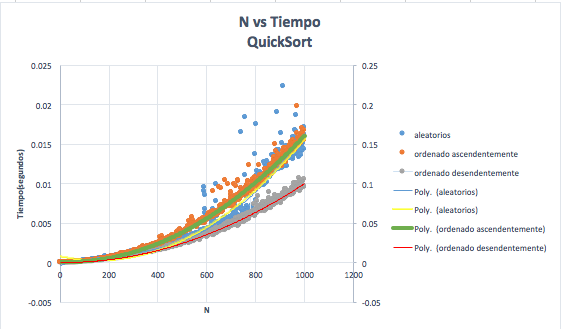
\includegraphics[scale=0.6]{Q}
\caption{Comportamiento algoritmo Quick Sort.}
\end{figure}

Este algoritmo es dependiente del pivote dado que el dividir del algoritmo es tan efectivo como la buena elección del pivote. Se escogió el pivote como el de más a la derecha para poder forzar el peor caso con un conjunto de datos específicos. Esto se nota en la gráfica ya que en el peor de los casos toma un tiempo mayor que en los otros dos en los cuales las particiones son más grandes lo cual reduce el tiempo de procesamiento del algoritmo.
\end{document}